
%(BEGIN_QUESTION)
% Copyright 2015, Tony R. Kuphaldt, released under the Creative Commons Attribution License (v 1.0)
% This means you may do almost anything with this work of mine, so long as you give me proper credit

The ``flare'' at an oil refinery functions as a safe way to quickly dispose of pressurized hydrocarbon compounds, by burning them far away from anything else that might be flammable.  In this system, as with most flare systems, a ``knockout drum'' exists to separate vapors from liquid, so that only vapors are sent to the flare tip to be burned.  Any captured liquid is drained to the Oily Water Sewer (OWS) system.  

Another vessel called the ``water seal drum'' maintains a column of water through which all flare gases must bubble through before passing on to the flare to be burned.  The purpose of the water seal drum is to prevent fire from possibly traveling backward through the process piping if ever a combustible mixture of fuel and oxygen were to exist in the flare system piping.  Water inside the seal drum is prevented from freezing in cold weather by a temperature control system located on that vessel:

Inspect this P\&ID closely to first identify all automatically-controlled valves, and then to predict whether a control valve with a linear inherent characteristic should behave linearly when installed (i.e. have a linear {\it installed} characteristic as well):

$$\includegraphics[width=15.5cm]{i0002rx01.eps}$$

\noindent
Assume the following parameters in this system:

\begin{itemize}
\item{} Flare gas temperature varies widely (from below ambient to hundreds of degrees Fahrenheit) depending on which units are discharging to the flare gas header at any time
\item{} PG-37 always registers atmospheric pressure (0 PSIG)
\item{} PG-36 varies from atmospheric (0 PSIG) to 35 PSIG, depending on how many units are discharging to that header pipe at any given time 
\item{} PG-35 always registers the same as PG-36
\item{} PG-12 varies between 85 PSIG and 25 PSIG depending on how fast water is being drawn to fill up the water seal drum
\item{} PG-10 reads nearly constant at 27 PSI all the time
\end{itemize}

\vskip 20pt \vbox{\hrule \hbox{\strut \vrule{} {\bf Suggestions for Socratic discussion} \vrule} \hrule}

\begin{itemize}
\item{} What is/are the decisive criteria for determining linear control valve behavior?
\item{} For any control valve in this process experiencing ``distortion'', what would you recommend we do to improve the control loop response?
\end{itemize}

\underbar{file i01379}
%(END_QUESTION)





%(BEGIN_ANSWER)

Did you think I would reveal details here and spoil your fun?

%(END_ANSWER)





%(BEGIN_NOTES)

The principle here is that any valve experiencing a flow-dependent pressure drop will need to have an equal-percentage (or suitably nonlinear) characteristic in order to perform linearly when installed.  Any valve lucky enough to experience a constant pressure drop under all flow conditions will work just fine with an inherently linear characteristic.

\vskip 10pt

TV-26 (steam heating valve) {\bf will respond linearly} with an inherently linear characteristic, because the steam supply pressure is constant as is the LP condensate line.

\vskip 10pt

LV-21 (water seal level valve) {\bf will not respond linearly} with an inherently linear characteristic, because its supply pressure falls off with flow rate.  An equal-percentage valve is recommended here.

\vskip 10pt

LV-24 (knockout drum condensate level valve) is {\bf uncertain} because we do not know how stable its pressure drop is as flow rate changes.  Some may try to base a conclusion on the variable flare line (and knockout drum) pressure, but this is irrelevant to the determination of valve characteristics because this pressure variability is not {\it flow-dependent}.  Pressure variances in the flare line are due to discharge conditions in the refinery units and not dependent at all on the flow rate through LV-24.

%INDEX% Documentation, loop diagram: realistic industrial example
%INDEX% Final Control Elements, valve: characterization
%INDEX% Process: flare knockout drum and water seal (realistic P&ID shown)

%(END_NOTES)


